%\documentclass[aps,prstab,showpac,twocolumn]{revtex4-1}  
\documentclass[aps,prstab,onecolumn,preprint]{revtex4-1}
%\documentclass[aps,prstab,onecolumn,preprint,endfloats,11pt]{revtex4-1}

\usepackage{graphicx}
\usepackage{epsfig}
\usepackage{subfigure}
\usepackage{fancyhdr}
\usepackage{color}
\usepackage{amsfonts}
\usepackage{amsmath}
\usepackage{amssymb}
\usepackage{dcolumn}
\usepackage{bm}
\usepackage{indentfirst}
\usepackage{rotating}
\usepackage{moreverb}



\linespread{1.0}

\makeatletter

\begin{document}

\title{Studies of Particle Motions During Slow Resonant Extraction}
\author{Chong Shik Park, James Amundson, Leo Michelotti, and Vladimir Nagaslaev}
\affiliation{Fermi National Accelerator Laboratory, PO Box 500, Batavia, IL 60510}
\date{\today}

\begin{abstract}
There are many interesting beam dynamics problems in third-integer resonant extraction. 
\end{abstract}

\pacs{}
%\maketitle

\setcounter{tocdepth}{7}

%\tableofcontents

\section{\label{sec:intro}Introduction}

%TODO
%need a table of all parameters of the extraction simulation, including dp/p


\section{\label{sec:bump}Local Orbit Corrections with Dynamic Bumps}

\subsection{\label{sec:bump0}Septum Entrance Angle}

In the previous paper~\cite{mu2e}, we discussed that a septum foil plane should be aligned with particles' entrance angles to the septum.
This alignment of the septum foil plane should be optimized in the manner of reducing particle losses due to crossing the plane from outside to inside a septum field region or vice versa.
In the Delivery Ring, however, the septum is placed at a zero dispersion section, and all shrinking separatrices are always centered at origin during extraction.
These yield that the Hardt condition, a condition to arrange separatrix geometries by superimposing them for different momenta, cannot be fulfilled~\cite{m.pullia}.
Consequently, particles' angle coordinates at the entrance of the first septum are not aligned with a fixed septum foil plane.

\begin{figure*}[!tbp]
  \subfigure[Before applying dynamic bumps]{
    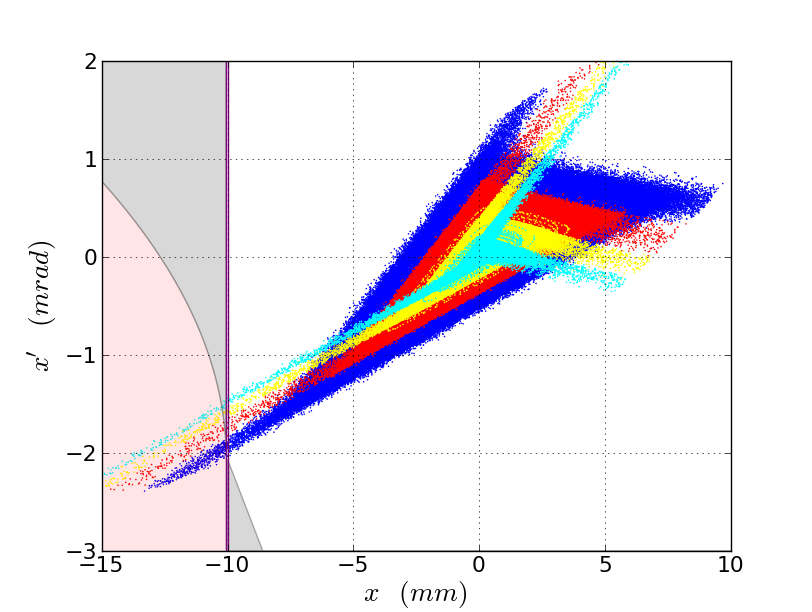
\includegraphics[width=.45\textwidth]{img/fig_bump1a.png}
    \label{fig:bump00}}
  \subfigure[After applying dynamic bumps]{
    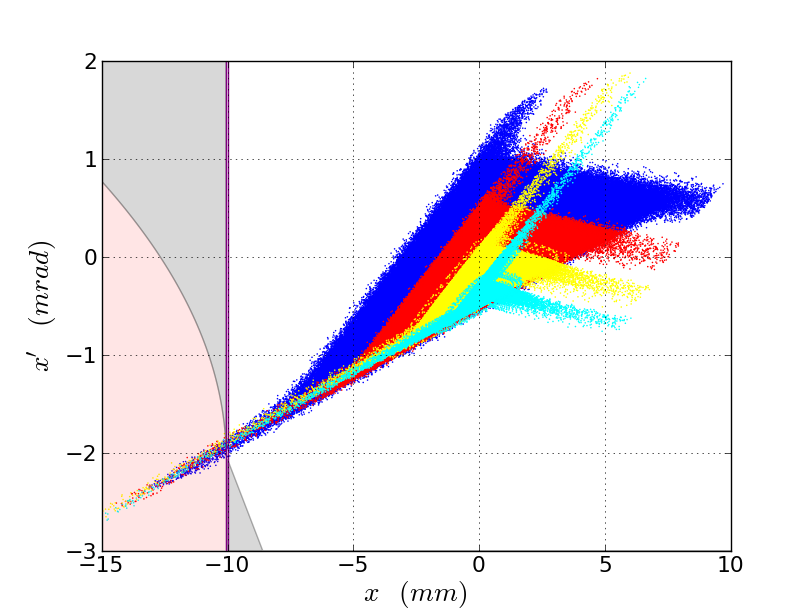
\includegraphics[width=.45\textwidth]{img/fig_bump1b.png}
    \label{fig:bump01}}
  \caption{\label{fig:bump0}Phase space plots of particles for 4 different extraction stages (turns 100(blue), 6000(red), 20000(yellow), and 30000(cyan)): (a) before and (b) after applying dynamic bump corrections. (Color: Red shaded part is the septum field region, and grey shaded one is the septum shadow regions.)}
\end{figure*}

Fig.~\ref{fig:bump00} shows a phase space of particles for four different extraction stages (turns 100, 6,000, 20,000, and 30,000).
As separatrix is squeezed by increasing tune-quad strengths, unstable particles are streamed along branches of separatrices. 
The septum field region (color: red shaded) is formed on the [left] side of the vertical septum foil line (color: purple) at $x=10$~mm. 
Gray shaded regions on the plot are defined as septum shadow regions in which particles will be considered as lost.
%The detailed explanation of the septum shadow regions is in Appendix~\ref{sec:shadow}.
Streams of unstable particles on the [leftmost] separatrix branch for each extraction stage are entering the septum field region by crossing the septum foil line.
However, their entering angles are moving [upward] during the extraction processes.
An angle of the septum foil plane is aligned with an initial extraction stage.
Therefore, the alignment is only valid for few turns at the beginning, and there will be continuous misalignment of the septum foil plane later.
These result that more particles are entering the [upper] septum shadow region (color:gray shaded), and they will be lost eventually.
Variations of angle coordinates at the septum entrance will be seen at the experiment target with a large horizontal angular spread of extracted beams.

In our case with the septum at a zero dispersion section, two possible ways can be considered to have same entrance angles of particles to the septum for different extraction stages.
The first method is to compensate the beam angle by rotating separatrices. This could be achievable by changing phases of two harmonic sextupole circuits.
The phase contributions of each harmonic circuit differs by about 90 deg, and these make phase adjustments doable.
However, particles' entrance angles for different extraction stages are same only if their $x$ coordinates are equal to the horizontal position of the septum foil at the entrance, $x_{ES}$.
In other words, their angles beyond $x_{ES}$ will be diverged.
These yield an asymmetric angular spread of extracted beams.

The other solution is to apply local orbit corrections using angle bumps throughout the spill.
Extracted particles will have a symmetric angular spread during the spill as well as same entrance angles.
For resonant extraction from the Delivery ring, we chose a local orbit correction scheme.
Particles' orbits in the extraction beamline will be dynamically corrected with four bump magnets.
As a backup solution to prepare a failure of local bump corrections, the harmonics sextupole magnets and their power supplies are designed to preserve ramp capabilities.
In this paper, we will only discuss how local bump corrections are implemented, and detailed specifications for magnets and power supplies are presented in the Mu2e TDR~\cite{tdr}.

\subsection{\label{sec:bump1}Dynamic Bumps}

\begin{figure}[!tbp]
  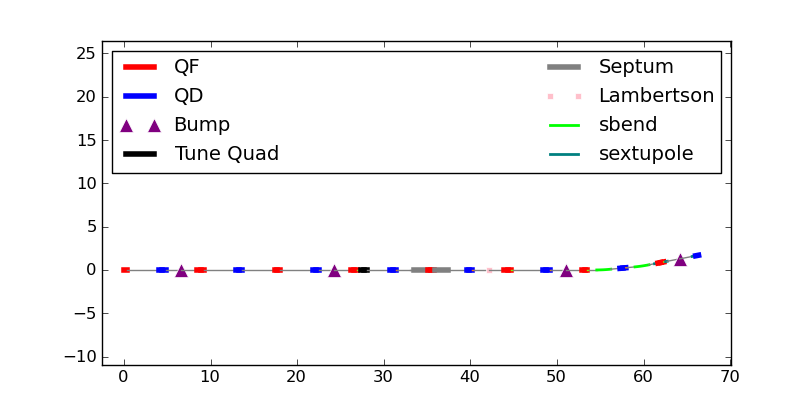
\includegraphics[width=.45\textwidth]{img/fig_bump2}
  \caption{\label{fig:bump1}Schematic drawing of the external beamline with four local orbit bumps.}
\end{figure}

Using four dynamic bumps, we could align separatrices to reduce angular deviations at the entrance of the septum.
Fig.~\ref{fig:bump1} is a schematic drawing of four dynamic bump locations in the extraction beamline.
Two bumps are located at the upstream of septa, and the other two are at the downstream.
Upstream bumps kick particles so that bases of separatrices are aligned during an entire extraction period.
Then, downstream bumps will kick them back to original orbits.
Fig.~\ref{fig:bump01} presents a phase space plot of particles for different extraction stages after applying local orbit corrections.
All triangular distributions of particles are well aligned on their bases.
The [leftmost] branch arms are extended to the same direction, i.e., particles are entering the septum field region with same anglular extensions.

Strengths of local orbit corrections can be easily obtained by applying a transfer matrix method with initial closed orbit conditions.
With the condition that the closed orbit is zero outside bumps, their strengths in time, $\theta_{i}(t)$ for $i=1,2,3,4$, are given by
\begin{equation}
  \begin{split}
  \theta_{1}(t) & = - \sqrt{\frac{\beta_{s}}{\beta_{1}}}
               \frac{\sin(\psi_{s} - \psi_{2})}
                    {\sin(\psi_{2} - \psi_{1})}
               \Delta x_{s}^{\prime} (t),
  \\ %\;\;\;
  \theta_{2}(t) & = \sqrt{\frac{\beta_{s}}{\beta_{2}}}
               \frac{\sin(\psi_{s} - \psi_{1})}
                    {\sin(\psi_{2} - \psi_{1})}
               \Delta x_{s}^{\prime} (t), \\
  \theta_{3}(t) & = \sqrt{\frac{\beta_{s}}{\beta_{3}}}
               \frac{\sin(\psi_{s} - \psi_{4})}
                    {\sin(\psi_{4} - \psi_{3})}
               \Delta x_{s}^{\prime} (t),
  \\ %\;\;\;\;\;\;\;\;\;\;
  \theta_{4}(t) & = - \sqrt{\frac{\beta_{s}}{\beta_{4}}}
               \frac{\sin(\psi_{s} - \psi_{3})}
                    {\sin(\psi_{4} - \psi_{3})}
               \Delta x_{s}^{\prime} (t),
  \end{split}
  \label{eqn:bump}
\end{equation}
where $\beta_{i}$'s are betatron functions at septum($s$) and bumps($1,2,3,4$), $\psi_{i}$'s are betatron phase advances, and $\Delta x^{\prime}_{s} (t)$ is required angle kick of particles at the septum entrance as a function of time.
Fig.~\ref{fig:bump2} shows changes of bump strengths vs.~time.
Since particles' entrance angles to the septum are aligned to the initial extraction stage, bump strengths are zero at the beginning and are maximum at the end of extraction.
From Eq.(~\ref{eqn:bump}), we observed that strengths of bump magnets would be getting smaller, when the distance of each pair for upstream and downstream bumps are closer.
Since each magnet is bounded between two quadrupoles, there are limitations in minimizing their strengths.

\begin{figure}[!tbp]
  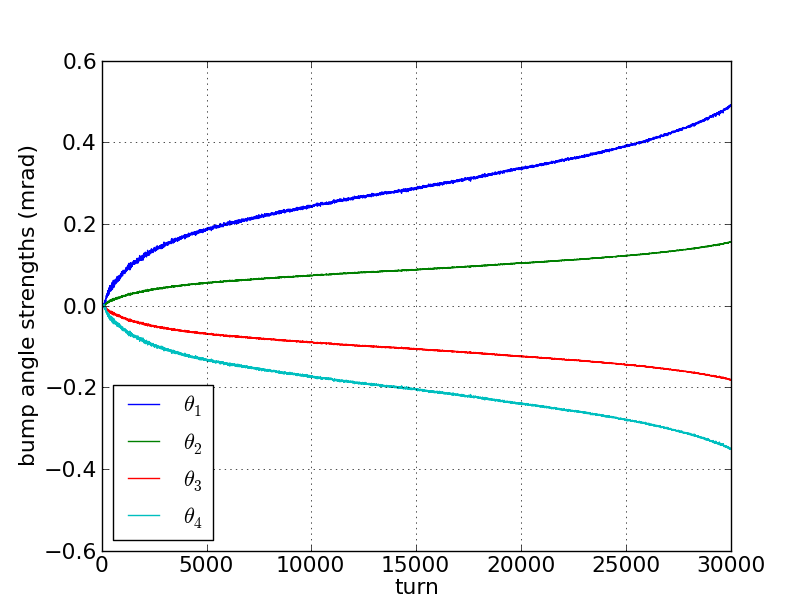
\includegraphics[width=.45\textwidth]{img/fig_bump3}
  \caption{\label{fig:bump2}Strengths changes of dynamic bumps in time.}
\end{figure}

\subsection{\label{sec:bump2}Simulation Results}

In Fig.~\ref{fig:bump3}, footprints of extracted particles at the entrance of the first septum are plotted in phase space coordinates.
These are accumulations of extracted particles with and without local orbit corrections throughout entire extraction period.
Particles (color: blue) survived from lost or scattered by the septum element will be transferred to the 2nd septum, a Lambertson magnet, and a C-magnet.
They will be then extracted to the external beamline.
Particles (color: black) formed a thin line on the [right] hit the septum foil with 50$\mu$m at the entrance during spill.
Some particles (color: red) intersect the septum foil plane by entering the septum shadow region (color: gray shaded).
The last two kinds of particles are removed and considered as lost in simulations.
The horizontal phase space ellipses (color: green), which match the beam with 99.9\% containment, are plotted alongside.

Before applying local orbit corrections, the footprint has a wider angular spread and there are many beam losses due to crossing the foil plane as seen in Fig.~\ref{fig:bump30}.
However, Fig.~\ref{fig:bump31} shows a narrower angular thickness of the extracted particle distribution with dynamic orbit corrections.
The footprint of the extracted beam without dynamic bumps is matched to an unnormalized emittance of [1.26]~$\pi$~mm-mrad and its matching horizontal betatron function is [9.1]~m. The local orbit corrected beam has a [0.55]~$\pi$~mm-mrad emittance and [20.1]~m betatron function.
After applying local orbit corrections, angular spreads of the beam also depend on the tune spread as the separatrix is squeezed.
The Delivery Ring has a nonzero chromaticity for the sufficient mixing of the coherent RFKO excitation~\cite{ipac11}.
Therefore, a chromatic tune spread causes a little spread of angle coordinates as seen in Fig.~\ref{fig:bump31}, while the overall emittance of the corrected beam is smaller compared to that of uncorrected beam.

\begin{figure*}[!tbp]
  \subfigure[Before applying dynamic bumps]{
    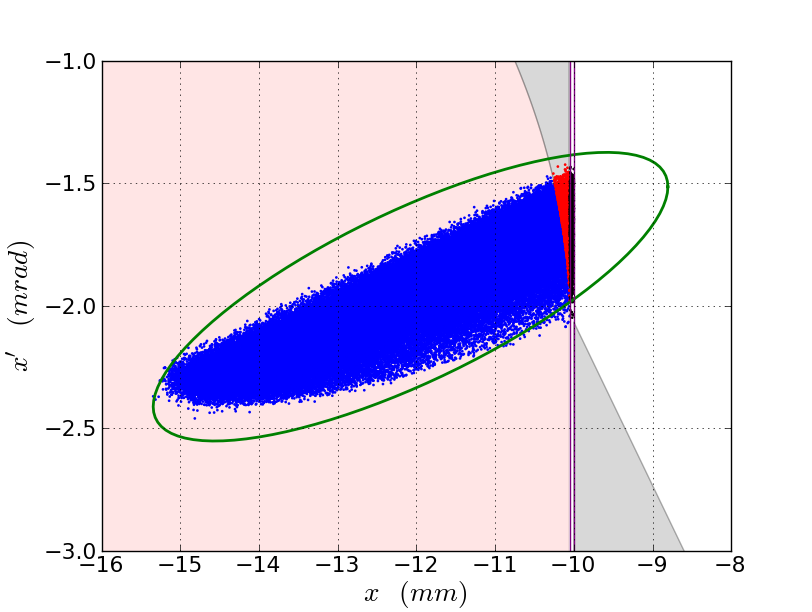
\includegraphics[width=.45\textwidth]{img/fig_bump4a}
    \label{fig:bump30}}
  \subfigure[After applying dynamic bumps]{
    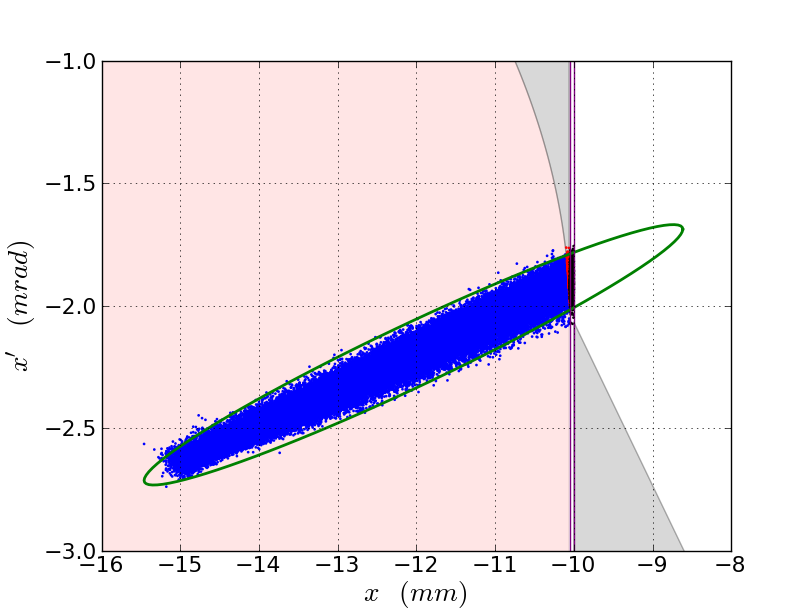
\includegraphics[width=.45\textwidth]{img/fig_bump4b}
    \label{fig:bump31}}
  \caption{\label{fig:bump3}Footprints of extracted particles with and without dynamic bumps. (Color: Blue dots are to-be-extracted particles, red dots are lost particles by intersecting the septum foil plane, and black dots are lost particles by hitting the septum. Red shaded part is the septum field region, and grey shaded one is the septum shadow regions.)}
\end{figure*}

As described in the previous paper~\cite{mu2e}, Synergia2 has a septum aperture to detect particle losses by hitting a septum head or crossing a septum foil plane.
The rotation of the septum plane is taken into account in the model.
Fig.~\ref{fig:bump4} shows extraction simulation results of particle losses with and without local orbit corrections during the spill.
While ``hit\_septum1'' and ``hit\_septum2'' are losses by hitting entrances of septum elements, ``cross\_septum1'' and ``cross\_septum2'' are losses by crossing septum foil planes for the 1st and 2nd septa, respectively.
``total\_losses'' are a sum of turn-by-turn particle losses for each turn.

Without dynamic angle corrections, septum planes are aligned only to the beginning of the extraction stage.
Therefore, beam losses are rising in time due to mismatching of the alignment (see Fig.~\ref{fig:bump40}).
When dynamic bumps correct beam orbits, particles' entrance angles are well matched to septum foil planes.
In Fig~\ref{fig:bump41}, turn-by-turn particle losses are not changing much and are much smaller compared with no orbit corrections.
We also observed that losses at the 2nd septum with dynamic bumps are decreased.

\begin{figure*}[!tbp]
  \subfigure[Before applying dynamic bumps]{
    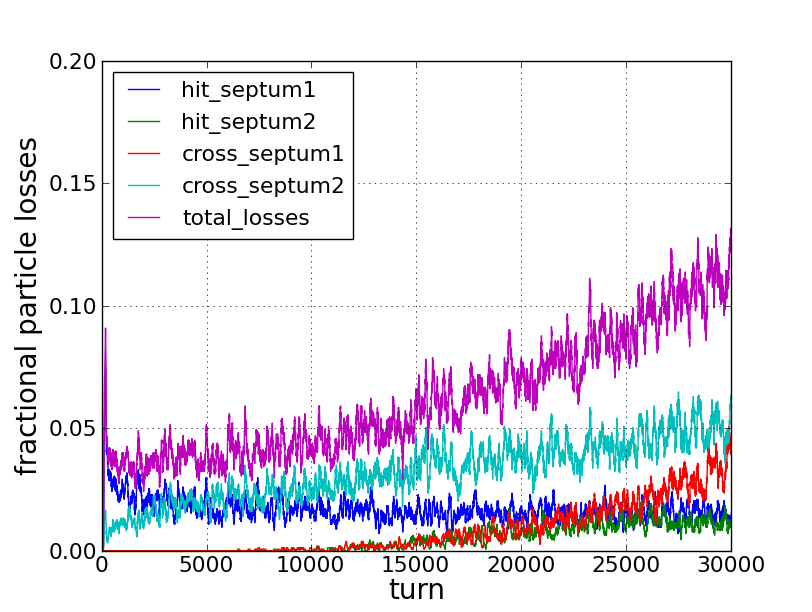
\includegraphics[width=.45\textwidth]{img/fig_bump5a}
    \label{fig:bump40}}
  \subfigure[After applying dynamic bumps]{
    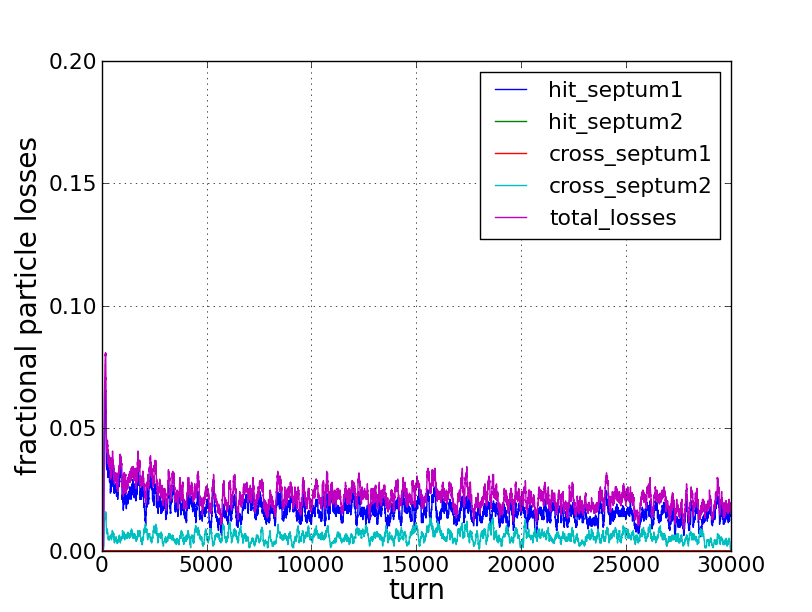
\includegraphics[width=.45\textwidth]{img/fig_bump5b}
    \label{fig:bump41}}
  \caption{\label{fig:bump4}Particle losses in time with and without dynamic bumps.}
\end{figure*}


\section{\label{sec:beamloss}Beam Loss Tracking}

After a bunch of particles enters a electrostatic septum element, a few particles will be have a chance scattered by a septum foil. Previous studies show that the chance are approximately $< 2 \%$. Synergia handle these particles as a beamloss. 

%TODO
%MARS parameters
%figure: MARS configuration
%figure: beamloss result


\section{\label{sec:arrival}Arrival Time Profile}



\section{\label{sec:rfko}Particle Motions with RFKO Beam Heating}

\subsection{\label{sec:dist}Beam Distribution Function}

\subsection{\label{sec:emit}Emittance Growth Rates}

\section{\label{sec:conclusion}Conclusion}

\section{\label{thanks}Acknowledgments}


% \appendix
% \section{\label{sec:shadow}The Septum Shadow Region}
% \subsection{Outside the Septum Field Region}
% \subsection{Inside the Septum Field Region}


\begin{thebibliography}{77}

  \bibitem{tdr}
  Mu2e Technical Design Documentation

  \bibitem{mu2e}
  C.S. Park, ``Tracking Simulation of the Third-Integer Resonant Extraction for the Fermilab Mu2e Experiment,'' submitted to PRST-AB.

  \bibitem{ipac11}
  V. Nagaslaev, J.F. Amundson, J.A. Johnstone, C.S. Park, and S.J. Werkema, ``Third Integer Resonance Slow Extraction Using RFKO at High Space Charge,'' in IPAC 2011 proceeding.

  \bibitem{m.pullia}
  M. Pullia, thesis

\end{thebibliography}

\clearpage

\end{document}

%sagemathcloud={"zoom_width":100}